% !TEX root =  ../main.tex
\section{Quarantine}

\subsection{Definition}

\subsubsection{Signature} \cstr{quarantine(s : set<server>)}

\begin{itemize}
\item \cstr{s} : an non-empty set of servers for a meaningful constraint. Servers not in the \st{Online} state are ignored.
\end{itemize}

The \cstr{quarantine} constraint disallows any VM running on servers other than those in \cstr{s} to be relocated into a server in \cstr{s}.
%
In addition, every VM running on a server in \cstr{s} cannot be relocated to another server.
%
This constraint only restricts the placement of running VMs with regards to a previous placement.
As a result, it is not possible to state for the satisfaction of one \cstr{quarantine} constraint before a reconfiguration occurred.

\classification{quarantine}{datacenter administrator}{VM placement}{VM-to-server placement,Partitioning,Maintenance}

\subsubsection{Usage}

A \cstr{quarantine} constraint may be use by the datacenter administrator for isolation purpose.
When a server appears to be compromised, a first step to avoid to propagate
the situation is to isolate it from the datacenter (put it into \emph{quarantine}).
Using one \cstr{quarantine} constraint, the datacenter administrator is ensured that
no running VMs may enter or leave the quarantine zone.

This constraint may also be used to prepare the servers for a software maintenance operation
when it is not possible to relocate the VMs it runs.
%
To prepare a software maintenance, the datacenter administrator must be sure the server
does not host any running VMs to prevent a misconfiguration from altering them. As their relocation
is not possible in this setting, the only solution to tend to have a server ready for the maintenance
is to wait for its VMs termination while disallowing other VMs to be running on the server.
The datacenter administrator may then use a \cstr{quarantine} constraint for that purpose.


\subsubsection{Example}

Figure~\ref{fig: quarantine} depicts a sample reconfiguration between a source and a destination configuration. In this example, the following \cstr{quarantine} constraints were considered:

\begin{itemize}

\item \cstr{quarantine(\{N2\})}. This constraint is satisfied as \cstr{VM3} was not relocated while no VMs
were moved or launched to \cstr{N2}.
\item \cstr{quarantine(\{N1,N4\})}. This constraint is satisfied as \cstr{VM2} is terminated
\item \cstr{quarantine(\{N3\})}. This constraint is not satisfied as \cstr{VM5} was launched on \cstr{N3} which is in the quarantine zone.
\end{itemize}

\begin{reconfiguration}
\centering
\begin{minipage}[b]{0.40\textwidth}
\begin{lstlisting}
N1: VM1 VM2
N2: VM3
N3: VM4
(N4):
?: VM5
\end{lstlisting}
\end{minipage}
\begin{minipage}[b]{2cm}
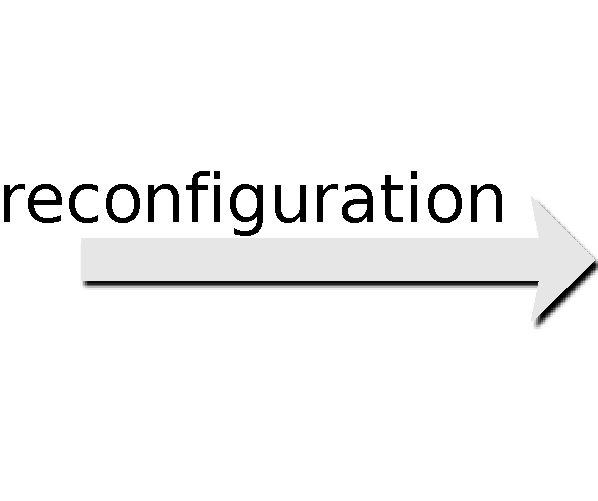
\includegraphics[width=2cm]{img/arrow_reconfiguration}
\end{minipage}
\begin{minipage}[b]{0.40\textwidth}
\begin{lstlisting}
N1: VM1
N2: VM3
N3: VM4 VM5
(N4):
?:
\end{lstlisting}
\end{minipage}
\caption{A reconfiguration motivated by \cstr{quarantine} constraints.}\label{fig: quarantine}
\end{reconfiguration}

\fullVersion{
\subsection{Model}

This constraint is modeled using domain restrictions on the demanding slice of the VMs.

\begin{equation*}
\begin{split}
\forall N \subset \mathcal{N}, \ quarantine(N) \triangleq&\\
&\forall v_i \in \mathcal{V} | v_i^h \in \bigcup_{j | n_j \in N}, d_i^h = c^h \\
&\forall v_i \in \mathcal{V} | v_i^h \ni \bigcup_{j | n_j \in N}, d_i^h \ni \bigcup_{j | n_j \in N}
\end{split}
\end{equation*}

\subsection{Violation Detection}

\subsection{Availability}
\subsubsection{In {\btrp}} 
This constraint is available in {\btrp} since the version 2.0 using the name \texttt{Quarantine}.
Using the global constraint catalog, the assignment of the d-slice placement variable in the quarantine
zone is restricted using \emph{in} constraints while VMs outside the quarantine zone are prevented to 
be relocated on the nodes in the quarantine using \emph{not\_in} constraints.

\begin{equation*}
\begin{split}
\forall N \subset \mathcal{N}, \ quarantine(N) \triangleq&\\
&\forall v_i \in \mathcal{V} | v_i^h \in \bigcup_{j | n_j \in N}, eq(d_i^h, c_i^h) \\
&\forall v_i \in \mathcal{V} | v_i^h \ni \bigcup_{j | n_j \in N}, not\_in(d_i^h, \bigcup_{j | n_j \in N})
\end{split}
\end{equation*}
}
\subsection{See also}

\subsubsection{Related Constraints}
\begin{itemize}
\item \cstrref{ban}: When it is possible to relocate the VMs, a \cstr{ban} constraint may be use to prepare servers for a software maintenance operation. In this setting, the server will be ready for the maintenance sooner as the VMs will be immediately relocated while the datacenter administrator has to wait for their termination when a \cstr{quarantine} constraint is used.

\item \cstrref{fence} $+$ \cstrref{root}. This composition of constraints
emulates a \cstr{lonely} constraint. One \cstr{fence} constraint will disallow the VMs outside the quarantine zone to enter it while one \cstr{root} constraint will prevent the relocation of the VMs running into the quarantine zone.

\item \cstrref{lonely}. A partitioning constraint to isolate VMs rather than servers.
\end{itemize}

\emulatedWith{quarantine}{fence,root}{\cstr{quarantine(s)}}{\cstr{root({\tuparrow}s), fence(\oline{{\tuparrow}s}, \oline{s})}}
\printListOfInheritance{quarantine}